\chapter{Постановка задачи о перераспределении потоков} \label{ch1}

При моделировании перераспределения потоков между трещинами автоГРП важно учитывать падение давления на трение в скважине $\Delta p_{fric}$ и падение давления на перфорациях $\Delta p_{perf}$.

На рис. \ref{fig:flow_distribution_scheme} представлена схема перераспределения потоков между тремя трещинами автоГРП.

\begin{figure}[H] 
\center
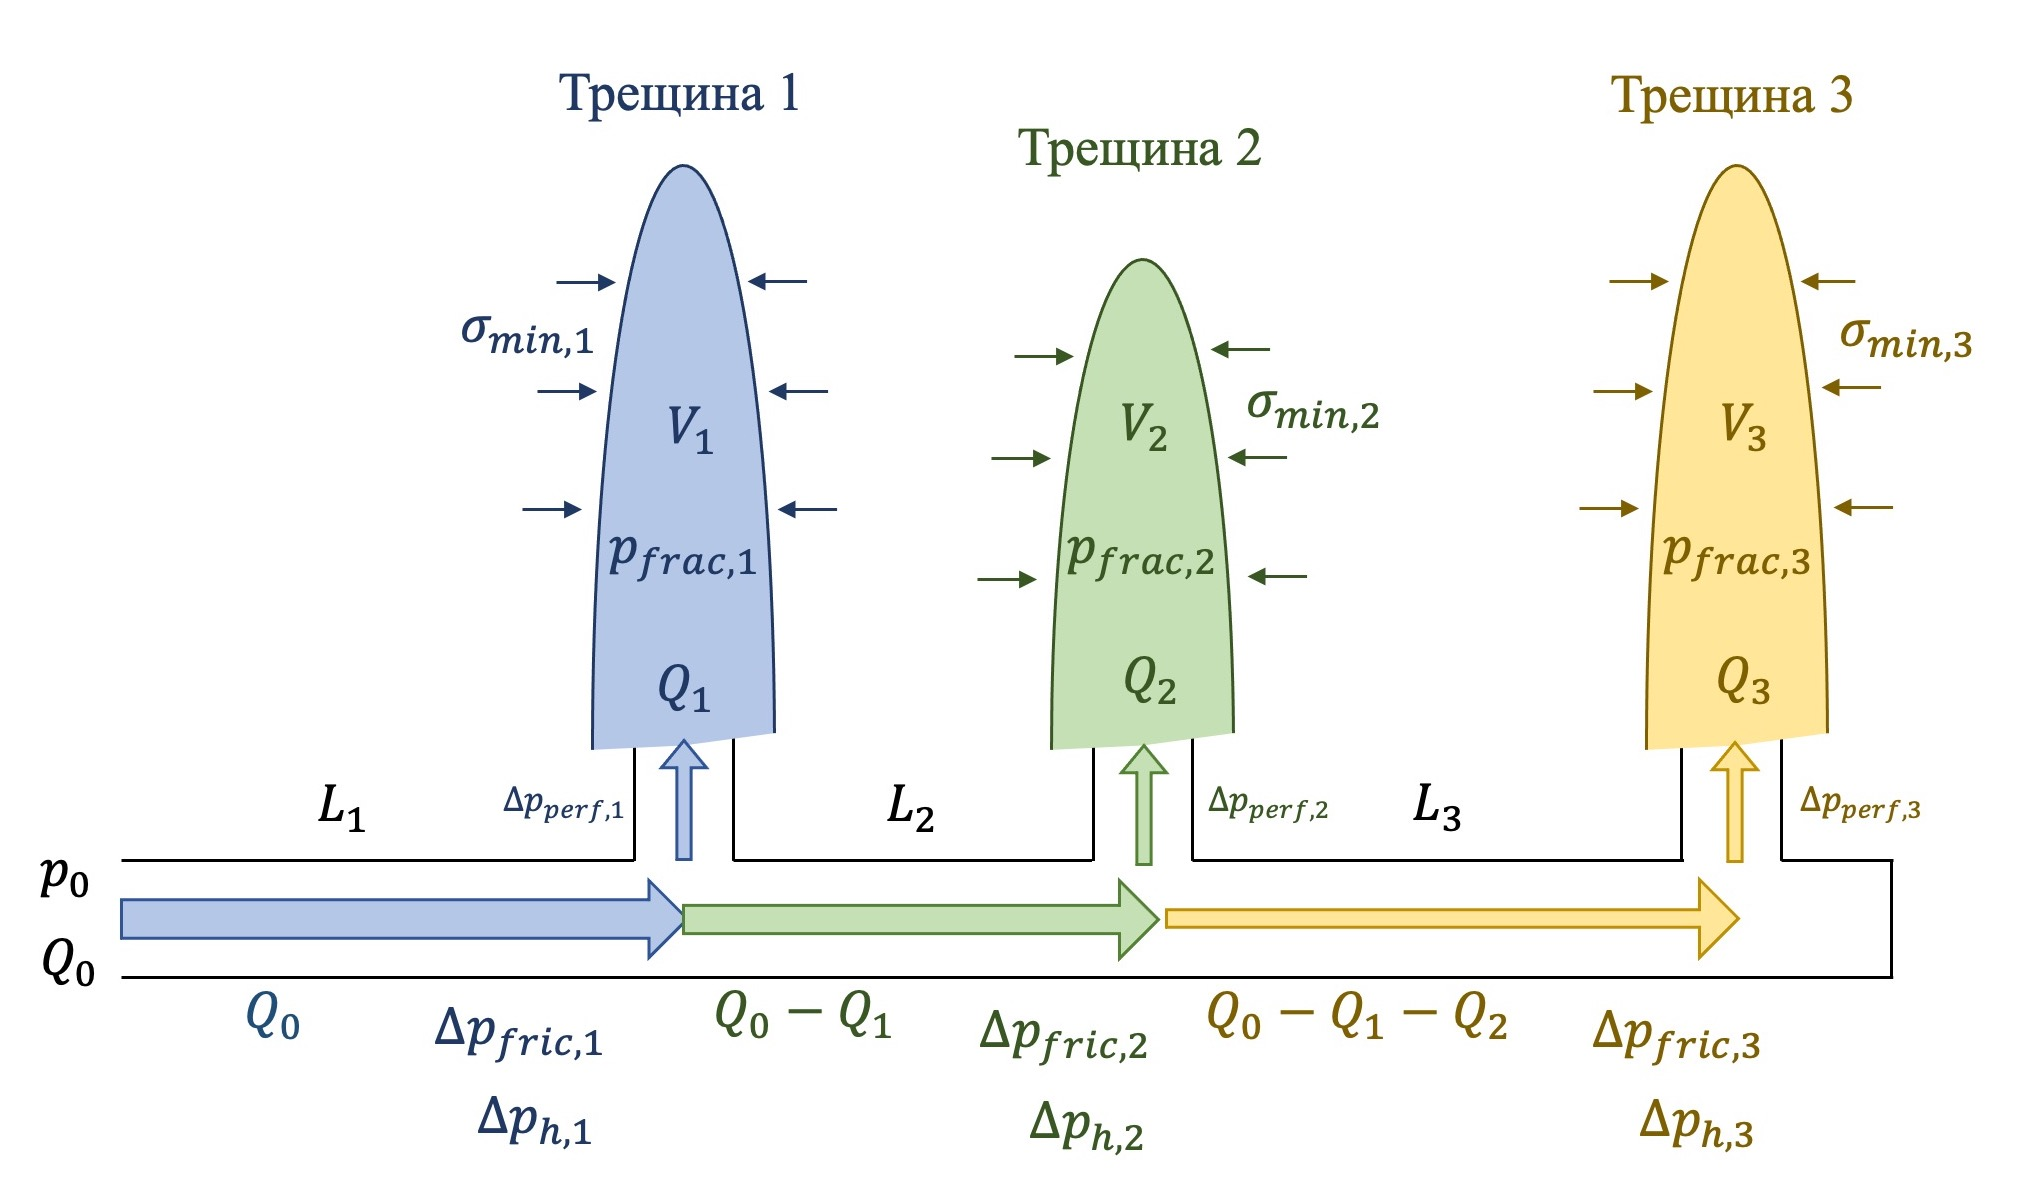
\includegraphics[width=0.9\linewidth]{images/flow_distribution_scheme.jpg}
\caption{Схема перераспределения потоков между трещинами гидроразрыва} 
\label{fig:flow_distribution_scheme}  
\end{figure}

Из рисунка \ref{fig:flow_distribution_scheme} видим, что весь расход, который закачиваем в скважину, перераспределяется между трещинами (первый закон Кирхгофа):
\beq\label{1_1}
Q_0=\sum\limits_{i=1}^{N}Q_i,
\eeq
где $N$ -- количество трещин.

Каждый из путей к каждой из трещин будем рассматривать независимо, т.е. будем считать гидродинамические сопротивления независимо (второй закон Кирхгофа):
\beq\label{1_2}
p_0=\sigma_{min,i}+p_{net,i}+\Delta p_{perf,i}-\sum_{j=1}^{i}{\Delta p_{h,j}}+\sum_{j=1}^{i}\Delta p_{fric,j},
\eeq
где $\sigma_{min,i}$ -- давление закрытия (минимальное напряжение в пласте) на $i$-ой трещине;\newline
$p_{net,i}=p_{frac,i}-\sigma_{min,i}$ -- чистое давление на $i$-ой трещине (из модели трещины);\newline
$\Delta p_{perf,i}$ -- падение давления вдоль перфорации $i$-ой трещины;\newline
$\Delta p_{h,i}$ -- падение гидростатического давления между $i$-ой и $(i-1)$-ой трещинами;\newline
$\Delta p_{fric,i}$ -- падение давления на трение между $i$-ой и $(i-1)$-ой трещинами.

Для PKN модели трещины гидроразрыва известна формула для чистого давления в трещине (подробное описание модели PKN приведено в следующем разделе):
\beq\label{1_3}
p_{net,i}(Q_i)=a_iQ_i^{\frac{n}{2n+3}}V_i^{\frac{1}{2n+3}},
\eeq
\ \\
где $a_i=\left(\dfrac{(n+3)(2n+1)^n \cdot K\cdot (E_i')^{2n+2}}{\pi\, 2^{2n}n^n\phi^n h_i^{3n+3}}\right)^{\!\frac{1}{2n+3}}$ -- параметр жёсткости,\newline\\
$Q_i$ и $V_i$ -- расход на $i$-ой трещине и объём $i$-ой трещины;\newline
$K$ и $n$ -- реологические параметры степенной (неньютоновской) жидкости;\newline
$E_i'$ -- модуль плоской деформации $i$-ой трещины;\newline
$h_i$ -- мощность продуктивной зоны.
\\

Эмпирическая формула для падения давления на перфорациях выглядит следующим образом:
\beq\label{1_4}
\Delta p_{perf,i}=\frac{8\rho_s}{\pi^2 C_{d,i}^2 n_{p,i}^2 d_{p_i}^4}Q_i\left|Q_i\right|,
\eeq
где $\rho_s$ -- средняя плотность смеси;\newline
$n_{p,i}, d_{p,i}$ -- количество и диаметр перфораций;\newline\\
$C_{d,i}=\dfrac{\text{min}(d_{jet})}{d_p}$ -- безразмерный коэффициент эррозии (в случае отсутствия твёрдых частичек в потоке $C_{d,i}\in\left[0.5,0.6\right]$, а с твёрдыми частичками в потоке $C_{d,j}\in\left[0.6,0.95\right]$  из-за эррозии перфорации).
\\

Падение давления на трение на каждом интервале рассчитывается по следующей формуле:
\beq\label{1_5}
\Delta p_{fric,i}=\int\limits_{x_{i-1}}^{x_i}{f\frac{\rho u_{m,i}^2}{R_i}}=\int\limits_{x_{i-1}}^{x_i}{\frac{\rho(c(t,s))\cdot f(Re)\cdot \left(Q_0-\sum\limits_{j=1}^{i-1}{Q_j}\right)^{\!2}}{R_i(s)S_i^2(s)}}ds,
\eeq
где $f=\dfrac{\tau}{\rho u_{m,i}^2/2}$ -- коэффициент трения Фаннинга;\newline\\
$\rho(c(t,s))$ -- плотность смеси, которая зависит от динамически меняющейся концентрации проппанта;\newline\\
$u_{m,i}=\dfrac{Q_0-\sum\limits_{j=1}^{i-1}{Q_j}}{S_i}$ -- средняя скорость на рассматриваемом участке трубы;\newline\\
$S_i$ -- площадь сечения рассматриваемого участка трубы;\newline
$R_i$ -- радиус рассматриваемого участка трубы;\newline
$Re$ -- число Рейнольдса.

Подставляя выражения \eqref{1_3}, \eqref{1_4} и \eqref{1_5}, в законы Кирхгофа \eqref{1_1} и \eqref{1_2}, получаем систему нелинейных алгебраических уравнений, которая может быть решена численно с помощью метода Ньютона.

В следующем разделе будут рассмотрены различные модели трещин гидроразрыва и их ограничения.
Будет выбрана наиболее подходящая модель для описания роста трещин автоГРП.



